\documentclass{beamer}

\usetheme{Frankfurt}
\usefonttheme{structureitalicserif}
\usecolortheme[RGB={203, 25, 52}]{structure}

\usepackage{graphicx}
\usepackage{pgf}
\usepackage{wrapfig}
\usepackage{amsmath}
\usepackage{amssymb}
\usepackage{gclc}
\usepackage[serbian]{babel}

\usepackage{amssymb}
\usepackage{gclc}
\usepackage{stmaryrd}
\usepackage{tikz}


\newcommand{\agbett}[3]{\ensuremath{\mathcal{B}_T^{\mathit{ag}}\ #1\ #2\ #3}}
\newcommand{\agbeth}[3]{\ensuremath{\mathcal{B}_H^{\mathit{ag}}\ #1\ #2\ #3}}
\newcommand{\agcongr}[4]{\ensuremath{#1#2 \cong^{ag} #3#4}}
\newcommand{\aginh}[2]{\ensuremath{#1 \in^{ag}_H #2}}
\newcommand{\agtransp}[2]{\ensuremath{transp^{ag}\ #1\ #2}}
\newcommand{\agtransl}[2]{\ensuremath{trans^{ag}_l\ #1\ #2}}
\newcommand{\agrotp}[2]{\ensuremath{rotp^{ag}\ #1\ #2}}
\newcommand{\agsymp}[1]{\ensuremath{symp^{ag}\ #1}}
\newcommand{\agrotl}[2]{\ensuremath{rotl^{ag}\ #1\ #2}}
\newcommand{\agsqdist}[2]{\ensuremath{d^2_{ag}\ #1\ #2}}



\newcommand{\bett}[3]{\ensuremath{\mathcal{B}_t(#1, #2, #3)}}
\newcommand{\colint}[3]{\ensuremath{\mathcal{C}_t(#1, #2, #3)}}
\newcommand{\congrt}[4]{\ensuremath{#1#2 \cong_t #3#4}}

\newcommand{\inh}[2]{\ensuremath{#1 \in_h #2}}
\renewcommand{\beth}[3]{\ensuremath{\mathcal{B}_h(#1, #2, #3)}}
\newcommand{\colinh}[3]{\ensuremath{\mathcal{C}_h(#1, #2, #3)}}
\newcommand{\congrh}[4]{\ensuremath{#1#2 \cong_h #3#4}}

\newcommand{\vect}[1]{\vec{#1}}

\def\d{{\fontencoding{T1}\selectfont\dj}}
\def\D{{\fontencoding{T1}\selectfont\DJ}}

\title{Prijava teze "Formalizacija razli\v citih modela geometrije i primene u formalizaciji automatskih 
dokaziva\v ca teorema"}

\author[Danijela Simi\'c]{Danijela Simi\'c\\{\small Mentor: prof. dr. Filip Mari\'c}}
\date[\today]{}

\begin{document}

\begin{frame}
\titlepage
\end{frame}

\section{Dokaziva\v ci teorema -- motivacija}

\begin{frame}{Za\v sto koristiti ra\v cunare za dokazivanje teorema?}
\begin{itemize}
\item Rigoroznost matemati\v ckih dokaza
\item Veliki broj gre\v saka u istoriji matematike
\item Problem nepotpunih definicija
\item Problem nekompletnih dokaza, sa namerno ili slu\v cajno izostavljenim delom dokaza
\item Problem recezenata
\end{itemize}
\end{frame}

\begin{frame}{Dokaziva\v ci teorema}
Sistemi za proveru dokaza:
\begin{itemize}
\item Automatski dokaziva\v ci 
\item Poluautomatski dokazava\v ci (asistenti za dokazivanje teorema)
\end{itemize}

Dokaziva\v ci teorema u geometriji:
\begin{itemize}
\item Aksiomatski dokaziva\v ci
\item Algebarski dokaziva\v ci
\end{itemize}
\end{frame}


\begin{frame}{Motivacija}
\begin{center}
\input{slika1.pic}
\end{center}
\end{frame}

\begin{frame}{Motivacija}
Formalizovati prelazak sa \structure{sinteti\v cke geometrije} na \structure{zapis u polininomima}:
\begin{itemize}
\item Formalizovati analiti\v cku geometriju, tj. pokazati da je analiti\v cka geometrija model geometrije Tarskog i Hilberta.
\item Formalizovati prevodjenje konstrukcija u polinome.
\end{itemize}
\end{frame}


\section{Formalizacija analiti\v cke geometrije}

\begin{frame}
\begin{itemize}
\item Postoji mnogo razli\v citih geometrija
\item Euklidska (sinteti\v cka geometrija): Euklidovi "Elementi", sistemi Tarskog, Hilberta i Avigadov sistem
\item Dekartov koordinatni sistem, uspostavlja vezu izme\d u sinteti\v cke geometrije i algebre
\item Postoji vi\v se poku\v saja da se formalizuje geometrija
\item Kori\v s\'cenje \structure{dokaziva\v ca teorema} pove\'cava se nivo rigoroznosti
\item Sistem Isabelle/HOL
\end{itemize}
\end{frame}

\begin{frame}{Formalizacija analiti\v cke geometrije}
\begin{itemize}
\item Formalizovana analiti\v cka geometrija u okviru dokaziva\v ca teorema.
\item Razli\v cite definicije istih pojmova su pokazane da su me\d usobno ekvivalentne
\item Formalizovano da analiti\v cka geometrija predstavlja model geometrije Tarskog i geometrije Hilberta (dokazane aksiome
      Tarskog i Hilberta u analiti\v ckoj geometriji).
\item U dokazima su kori\v s\'cenje izometrijske transformacije, radi upro\v s\'cavanja dokaza
\item Na\v sa formalizacija se zasniva na aksiomama realnih brojeva i osobine realnih brojeva su kori\v s\'cene 
u dokazima
\end{itemize}
\end{frame}


\begin{frame}{Formalizacija analiti\v cke geometrije}
\begin{itemize}[<+->]
\item \structure{objekti:} ta\v cke (par realnih brojeva $\mathbb{R}^2$), prave
\item \structure{relacije:} incidencija, izme\d u, kongruencija
\end{itemize}
\end{frame}


\begin{frame}{Formalizacija analiti\v cke geometrije -- relacija izme\d u}
\begin{itemize}
    \item Relacija \structure{\emph{izme\dj u}}: $\mathcal{B}(A, B, C)$
    \item Aksiomatizacija \structure{Tarskog} dozvoljava jednakost me\d u ta\v ckama:
      \begin{block}{}
	   {\tt
	    \begin{tabbing}
	    \hspace{5mm}\=\hspace{5mm}\=\kill
	    $\agbett{(xa, ya)}{(xb, yb)}{(xc, yc)} \longleftrightarrow$\\
	    \>$(\exists (k::real).\ 0 \le k \ \wedge\ k \le 1 \ \wedge$\\
	    \>\>$(xb - xa) = k \cdot (xc - xa) \ \wedge\ (yb - ya) = k \cdot (yc - ya))$
	    \end{tabbing}
	    }
      \end{block}
  \end{itemize}
\end{frame}

\begin{frame}{Formalizacija analiti\v cke geometrije -- prave}
\begin{itemize}
    \item $A\cdot x + B\cdot y + C = 0$ where $A \neq 0 \vee B \neq 0$
    \item {\em ista prava}:
	\begin{description}
	  \item[-] $A\cdot x + B\cdot y + C = 0$ 
	  \item[-] $k\cdot A\cdot x + k\cdot B\cdot y + k\cdot C = 0$,
	      za realno $k \neq 0$
	\end{description}
\end{itemize}
	\begin{block}{Prava}
	  {\tt
	  \begin{tabbing}
	  Klasa ekvivalencije nad skupom\\
	  \hspace{5mm}$\{((A::real), (B::real), (C::real)).\ A \neq 0 \vee B \neq 0\}$
	  \end{tabbing}
	  }
	\end{block}
\end{frame}


\begin{frame}{Formalizacija analiti\v cke geometrije -- wlog}
 \begin{block}{Bez gubitka na op\v stosti}
    {\tt
    \begin{tabbing}
    $inv\ P\ t \longleftrightarrow (\forall\ A\ B\ C.\ P\ A\ B\ C \longleftrightarrow P\ (t A)\ (t B)\ (t C))$
    \end{tabbing}
    }
  \end{block}
  \begin{itemize}
    \item John Harrison, \emph{Without loss of generality}
  \end{itemize}
\end{frame}

\section{Formalizacija geometrije kompleksne ravni}

\begin{frame}{Poinkareov disk model}
\begin{center}
\input{slika2.pic}
\end{center}
\end{frame}

\begin{frame}{Poinkareov disk model - Prava} 
\begin{center}
\input{slika3.pic}
\end{center}
\end{frame}

\begin{frame}{Poinkareov disk model - Prava} 
\begin{center}
\input{slika4.pic}
\end{center}
\end{frame}

\begin{frame}{Poinkareov disk model - Izme\d u} 
\begin{center}
\input{slika5.pic}
\end{center}
\end{frame}

\begin{frame}{Poinkareov disk model - Izme\d u} 
\begin{center}
\input{slika6.pic}
\end{center}
\end{frame}


\begin{frame}{Poinkareov disk model - Izme\d u} 
\begin{center}
\input{slika7.pic}
\end{center}

Da li va\v zi: $\sphericalangle AOC = \sphericalangle AOB + \sphericalangle COB$
\end{frame}


\begin{frame}{Kompleksna geometrija}
\begin{itemize}[<+->]
\item Zamenom Dekartove ravni sa kompleksnom ravni dobijaju se kompaktnije i manje kompleksne formule.
\item Kompleksna ravan ili neki njen deo (jedini\v cni disk ili gornja poluravan) se \v cesto uzimaju kao 
      domen u kojima se formalizuju modeli razli\v citih geometrija.
\item Postoji potreba za formalizacijom
\item Postoji vi\v se pristupa u izlaganju materije u knjigama
\end{itemize}
\end{frame}


\begin{frame}{Glavni rezultati u formalizaciji kompleksne geoemtrije}
\begin{itemize}[<+->]
\item Pro\v sirena kompleksna ravan, dodata je ta\v cka $\infty$
\item Homogene koordinate:
      $$z = \frac{z_1}{z_2}$$
      pri \v cemu $z_1, z_2 \neq 0$ \\
      Jo\v s posmatramo i ovo:
      $$z = \frac{k\cdot z_1}{k \cdot z_2}$$
      pri \v cemu $k \neq 0$ \\
      Uvodimo relaciju $\approx$: $(z_1, z_2) \approx (k\cdot z_1, k\cdot z_2)$ 
i posmatramo \structure{klasu ekvivalencije} ove relacije nad skupom ne-nula vektora.
\end{itemize}
\end{frame}

\begin{frame}{Glavni rezultati u formalizaciji kompleksne geometrije}
\begin{itemize}[<+->]
\item $\infty = \frac{1}{0}$ -- klasa ekvivalencije elementa (1, 0) nad skupom ne-nula vektora
\item Uvodimo aritmeti\v cke operacije i pokazujemo da su dobro definisane, 
pokazujemo osnovna svojstva konjugata i inverzije
\item Defini\v semo dvorazmeru: 
      $$(z, u, v, w) = \frac{(z-u)(v-w)}{(z-w)(v-u)}$$
      i pokazujemo osnovna svojstva     
\end{itemize}
\end{frame}


\begin{frame}{Rimanova sfera i stereografska projekcija}
\begin{figure}[!h]
\begin{center}
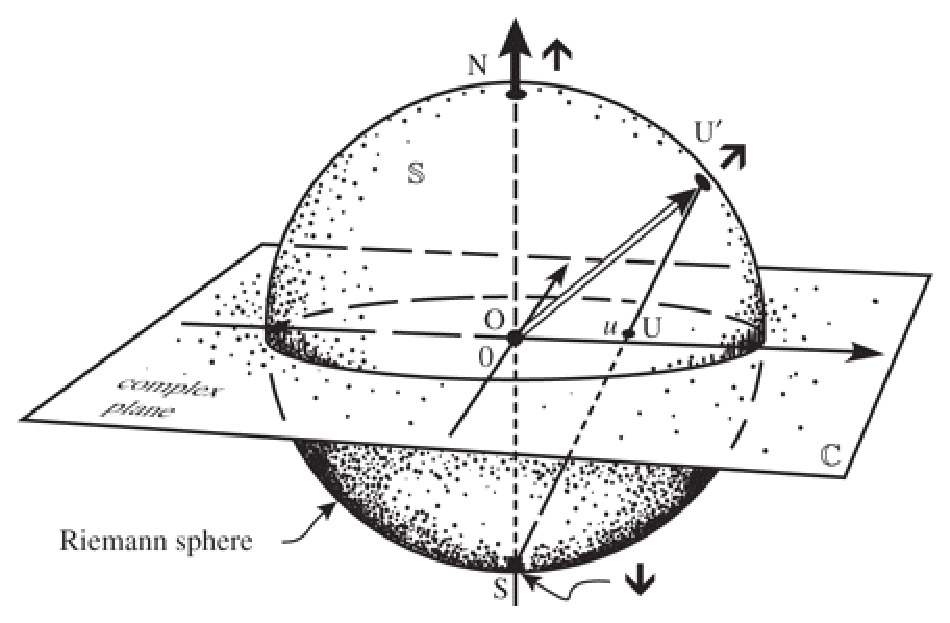
\includegraphics[width=0.6\textwidth]{riman.eps}
\end{center}
\end{figure}
\end{frame}

\begin{frame}{Mebijusove transformacije}
$$M(z) = \frac{a\cdot z + b}{c\cdot z + d}$$
$[M] = \begin{bmatrix} 
a & b \\
c & d
\end{bmatrix}$ pri \v cemu $|[M]| \neq 0$
\begin{itemize}[<+->]
\item Proporcionalne matrice predstavljaju jednu te istu Mebijusovu 
transformaciju
\item \structure{Kompozicija} Mebijusovih transformacija se dobija kao proizvod 
matrica koje ih predstavljaju
\item \structure{Inverzna} Mebijusova transfomacija se dobija kao inverzna 
matrica matrice koja predtavlja transformaciju
\item Dejstvo Mebijusa na ta\v cke:
      $$M(z) \longleftrightarrow \begin{bmatrix} a & b \\ c & d \end{bmatrix} 
\cdot \begin{bmatrix} z_1 \\ z_2 \end{bmatrix}$$
\end{itemize}
\end{frame}

\begin{frame}
\begin{itemize}
\item Pokazujemo da je dvorazmera Mebijusova transformacija i to 
koristimo da poka\v zemo da:
\item $z_1 \rightarrow$
\item $z_2 \rightarrow$
\item $z_3 \rightarrow$
\end{itemize}
\end{frame}

\begin{frame}
\begin{itemize}
\item Pokazujemo da je dvorazmera Mebijusova transformacija i to 
koristimo da poka\v zemo da:
\item $z_1 \rightarrow 0$
\item $z_2 \rightarrow 1$
\item $z_3 \rightarrow \infty$
\end{itemize}
\end{frame}

\begin{frame}
\begin{itemize}
\item Pokazujemo da je dvorazmera Mebijusova transformacija i to 
koristimo da poka\v zemo da:
\item $z_1 \rightarrow 0$
\item $z_2 \rightarrow 1$
\item $z_3 \rightarrow \infty$
\end{itemize}
\begin{block}{Bez gubitka na op\v stosti}
\begin{itemize}
\item[-] ako svojstvo P va\v zi za ta\v cke 0, 1 i $\infty$
\item[-] Mebijusova transformacija \v cuva svojstvo P
\item[-] \structure{zaklju\v cak:} svojstvo P va\v zi za bilo koje tri razli\v 
cite ta\v cke $z_1$, $z_2$ i $z_3$
\end{itemize}
\end{block}
\end{frame}

\begin{frame}{Uop\v steni krug}
Uop\v steni krug: mo\v ze biti prava, ali i krug
  $$A\cdot z \cdot \overline{z} + B \cdot \overline{z} + C \cdot z + D = 0$$
  $H = \begin{bmatrix} A & B \\ C & D \end{bmatrix}$ pri \v cemu $B = 
\overline{C}$ i $A, D \in \mathbb{R}$
\structure{$$\begin{bmatrix} z_1 z_2 \end{bmatrix}\begin{bmatrix} A & B \\ C & 
D \end{bmatrix}\begin{bmatrix} z_1 \\ z_2 \end{bmatrix} = 0$$}
\begin{itemize}
\item Svaki uop\v steni krug odgovara krugu na Rimanovoj sferi.
\end{itemize}
\end{frame}

\begin{frame}{Mebijusova transformacija uop\v stenog kruga}
$M$ -- Mebijusova transformacija (zadata matricom)\\
$H$ -- Uop\v steni krug (zadat Matricom) 
\structure{$$\text{adj} M^{-1}\cdot H\cdot M^{-1}$$}
\end{frame}

\begin{frame}{O\v cuvanje ugla}
\begin{figure}[!h]
\begin{center}
\includegraphics[width=1.0\textwidth]{Konformno.eps}
\end{center}
\end{figure}

$$\cos \angle H_1H_2 = \frac{|H_{1,2}|}{\sqrt{|H_1|}\sqrt{|H_2|}}$$
\end{frame}

\begin{frame}{Statistika formalizacije kompleksne geometrije}
\begin{itemize}
\item Broj definicija: oko 200
\item Broj teorema: oko 800
\item Broj linija koda: preko 13000
\end{itemize}
\end{frame}

\begin{frame}{Poincareov disk model}
Primene formalizacije kompleksne geometrije na Poincareov disk model: 
\begin{itemize}
\item definicija izme\dj u -- kori\v s\'cenjem dvorazmere
\item izometrijske transformacije koje slikaju unutra\v snjost diska u unutra\v snjost diska
\item rastojanje me\dj u ta\v ckama
\end{itemize}
\end{frame}

\section{Primena algebarskih metoda u stereometriji}

\begin{frame}{Primena algebarskih metoda u stereometriji}
\begin{itemize}
\item Predstaviti stereometrijske objekte u vidu algebarskih formula.
\item Primeniti na njih Vu-ov metod ili metod Grebnerovih baza
\end{itemize}
\end{frame}

\section{Zaklju\v cak}

\begin{frame}
Ostvareni ciljevi:
\begin{itemize}
\item Formalizacija analiti\v cke geometrije
\item Formalizacija geometrije kompleksne ravni
\item Deo formalizacije automatskog dokaziva\v ca teorema zasnovanog na Vu-ovoj metodi ili na metodi 
Grebnerovih baza 
\end{itemize}

Planirani ciljevi:
\begin{itemize}
\item Primena algebarskog dokaziva\v ca na probleme u stereometriji
\item Formalizacija Poinkareovog disk modela
\end{itemize}
\end{frame}

\end{document}



































